\chapter{Results}
\label{ch:results}

% TODO - revise chapter intro
This chapter follows the established pattern of qualitative,
bridging, and quantitative sections.


\section{A Qualitative Yolngu Seasonal Calendar}

The qualitative results fall into three parts.
%
First, personal reflections on my approach to interviews and drawing
from Indigenous knowledge - and how I underestimated the complexity
of seasonal calendars.
%
Second, a Yolngu seaonal calendar drawn from interview responses,
defining a handful of meteorologically-defined seasons each year.
This calendar is aligned with \textit{Man of All Seasons} \citep{davis1989},
and consistent with grey literature.
%
Third, commentary on how to accurately characterise Yonlgu seasons.
This section covers required datasets, historical changes, spatial
variation in definitions, and three distinct types of season.



\begin{figure}[h]
    \centering
    \includegraphics[width=\textwidth]{yolngu-calendar.jpg}
    \caption[Conceptual Yolngu seasonal calendar \citep{davis1989}]{
        Conceptual Yolngu seasonal calendar \citep{davis1989}
        NOTE - non-final version of figure; will redraw with circle only.}
    \label{fig:yolngu-seasons}
\end{figure}


\subsection{Reflection - Complex Calendars as an emergent theme}

`Calendar' and `season' are not concepts that translate directly across cultures. 

Discuss how I realised this, by re-listening to recordings, and that I was
expecting something unforeseen (but not like this!).

Note that informal, collaborative and participant-led conversations were key.

\emph{TODO: expand points to paragraphs, with quotes}

\begin{itemize}
\item all in english
\item what is a season
\item what is a calendar
\item there is no ``the'' yolngu calendar - varies spatially,
        multiple seasonal calendars for different temporal scales with varied purposes
\item `simple fact-finding' really isn't!
\item unusual or extreme events people remember, and how these fit into the calendar
\item understandings of climate change including expected impacts (minimal, after \citet{petheram2010})
\end{itemize}



\subsection{Yolngu Seasons vary by location and temporal scale}

Yolngu participants discussed seasons at three distinct temporal scales
each year, each type recognised by different indicators.

Each year, there is a wet season and a dry season.  These seasons are
recognised by the monsoon winds from the north-west and south-east
respectively.  Some years have a gap-filling season between them.

\begin{itemize}
\item `Monsoon seasons' - Wet and Dry - are recognised not by rainfall but
        by winds from the north-west and south-east respectively.
\item The six `weather seasons' are defined primarily by wind, rain, and temperature.
        They can begin and end at any time during the year - weather permitting -
        and may occur more than once and in any order.
\item Complex `ecological seasons', where changes in plant or animal life
        signal appropriate activities for that time.  A particular community
        may recognise tens of these, all highly localised.
\end{itemize}

A similar three-level pattern of seasons is visible in \autoref{fig:tiwi-seasons}.
The Tiwi seasons are shown at a monsoonal level, as well as by weather or ecology.
The latter categories are not clearly distinct in this figure.



\begin{landscape}
\begin{figure}[p]
    \centering
    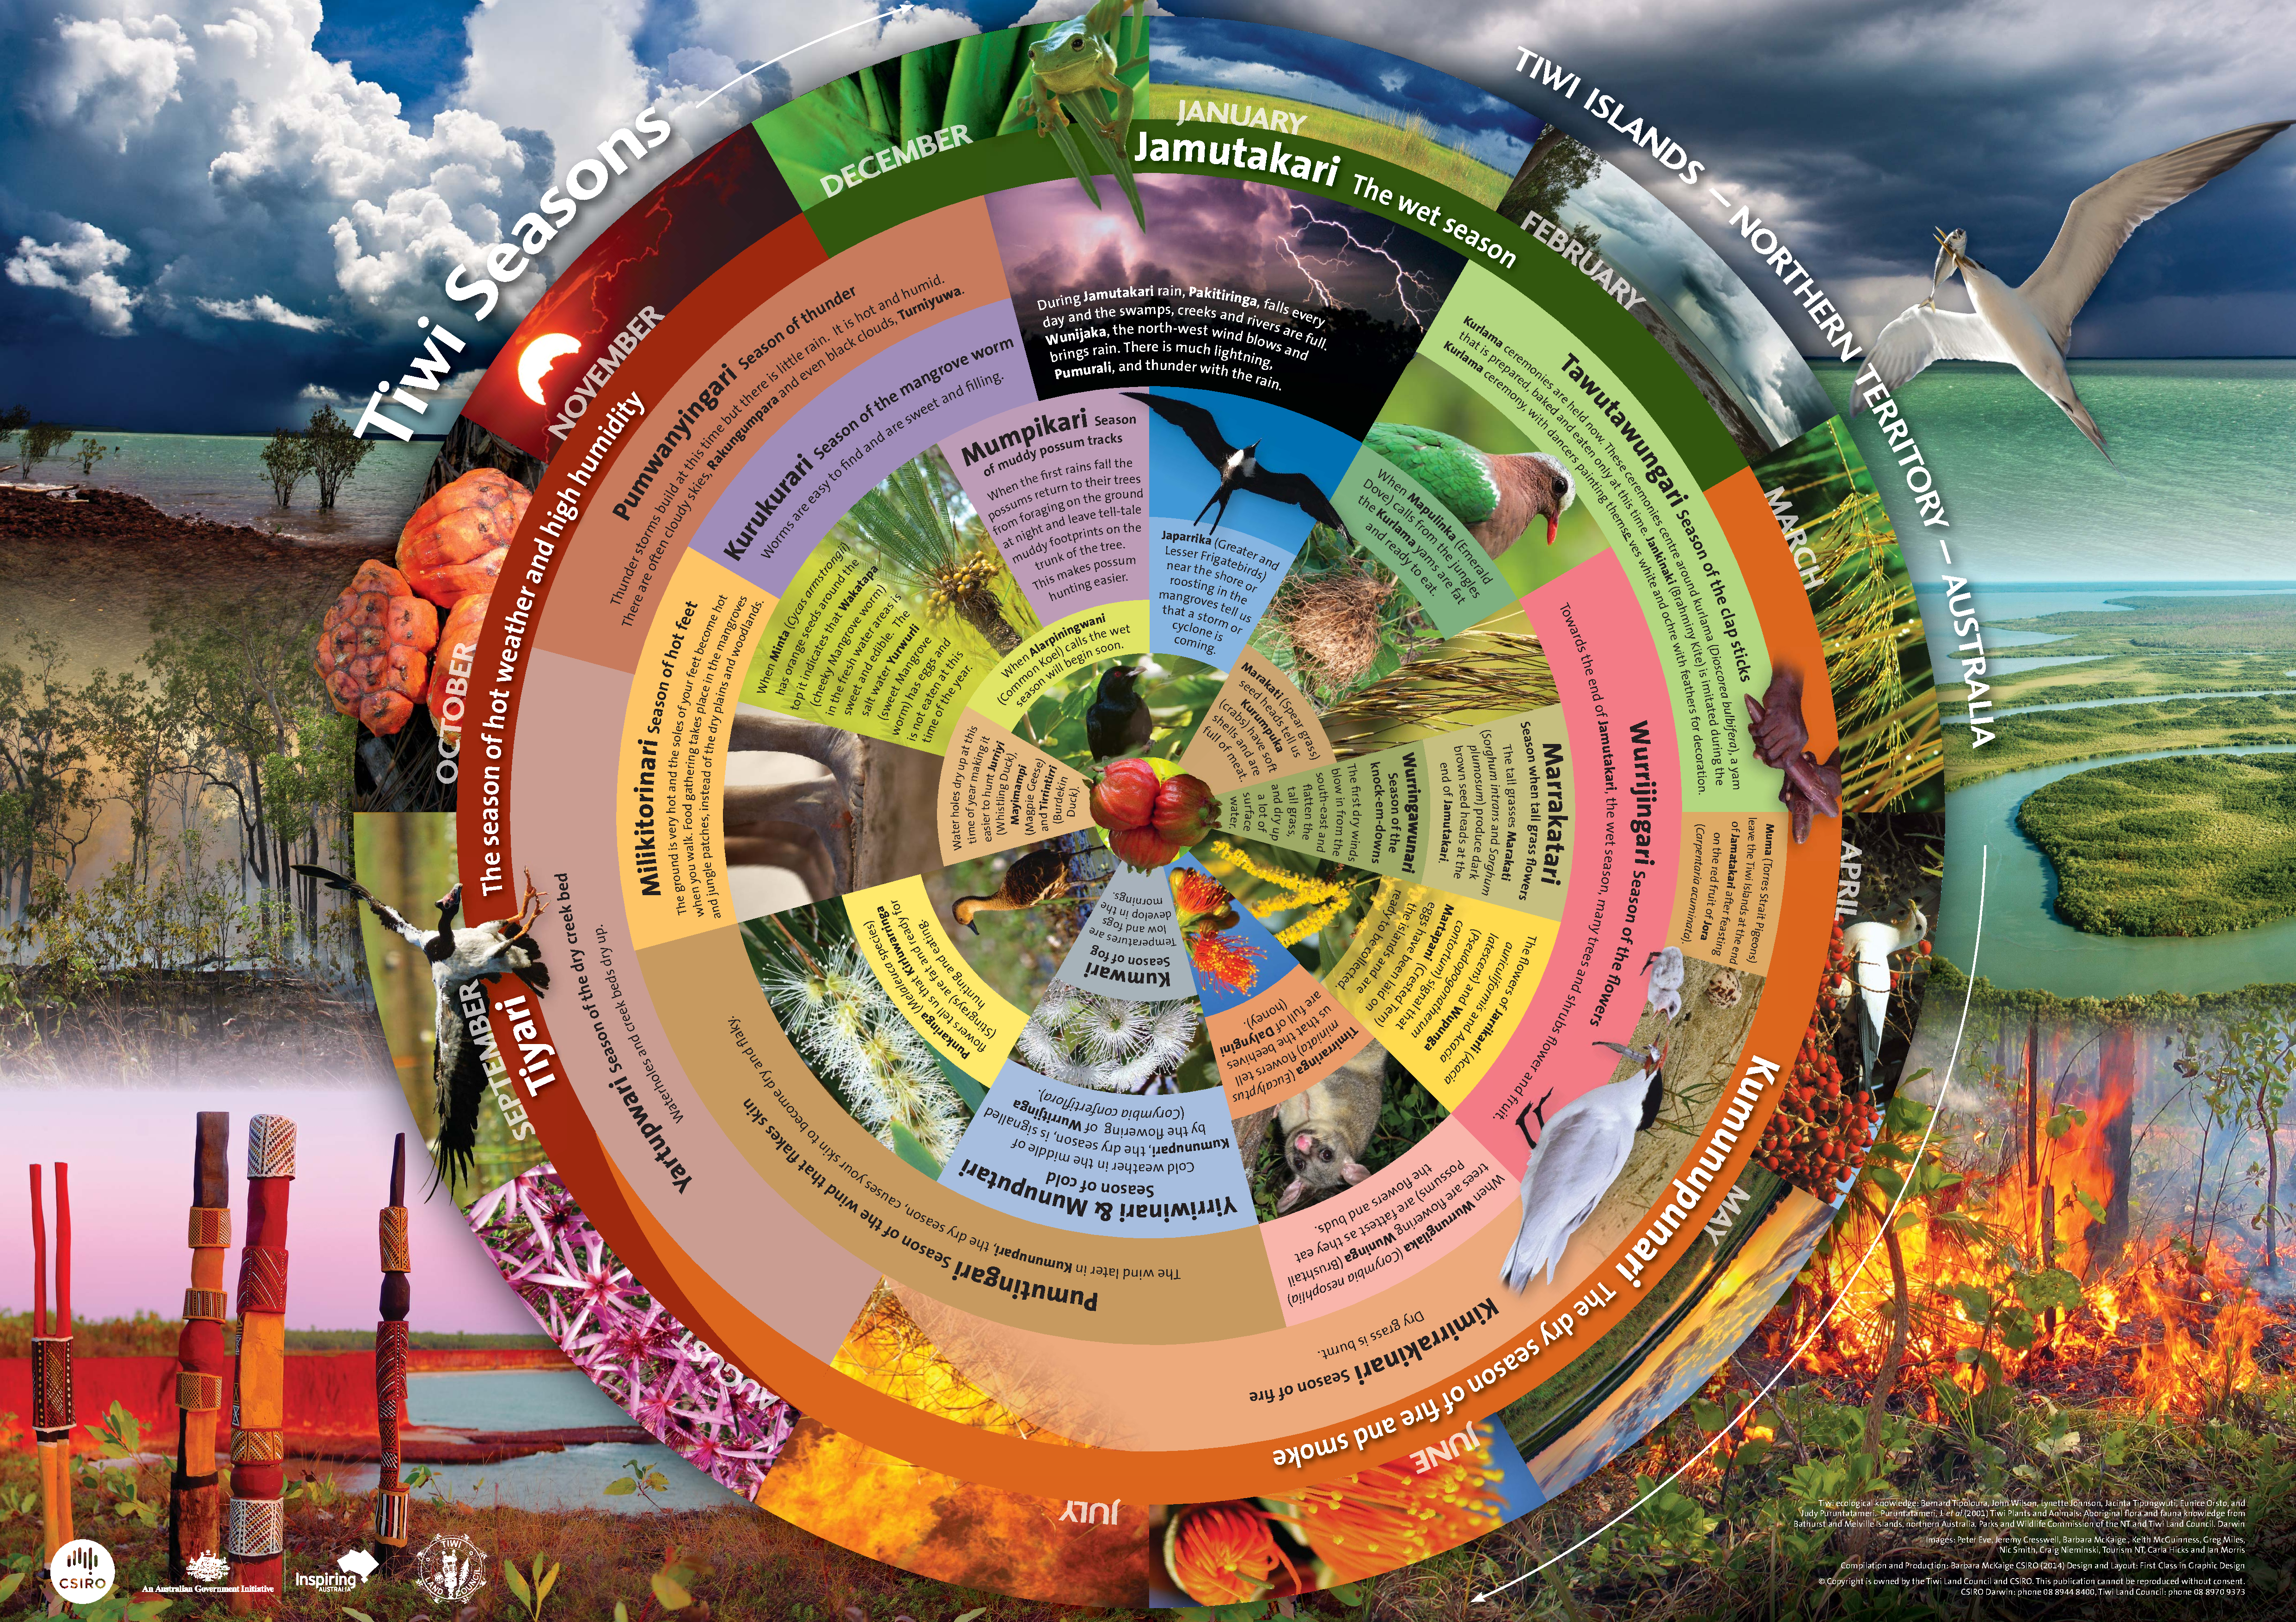
\includegraphics[width=\paperwidth]{TiwiSeasons.pdf}
    \caption[The Tiwi Seasons Calendar \citep{CSIROcals}]{
        The Tiwi Seasons Calendar \citep{CSIROcals}.
        This calendar shows month of year in the outermost ring,
        then three `major' Tiwi seasons recognised by weather.
        Note that \textit{Kumunupunari} does not have a sharp boundary with \textit{Tiyari}!
        Within this ring are smaller seasons, recognised by weather
        or ecological events and associated with particular activities.
        This format is designed for the circle to rotate, encouraging interaction or observation.
        }
    \label{fig:tiwi-seasons}
\end{figure}
\end{landscape}


\paragraph{Monsoon Seasons (Wet/Dry)}

Of the three levels of seasons recognised by Yolngu,
the wet/dry monsoon seasonal cycle is most likely familiar to non-Indigenous people -
especially in the tropics.  Yolngu participants emphasised that these seasons
are \emph{not} recognised by rainfall, but rather the direction of prevailing winds.

\blockquote{
    ADD QUOTE HERE
}

Interestingly, this mirrors the meteorological definition of monsoon,
where rainfall is less important than the location of the intertropical
convergence zone and consequent direction of prevailing wind.
This shared understanding of monsoon seasonality should not go unremarked -
but does direct this research to the more local seasonal patterns.


\paragraph{Meteorological Seasons}

Lorem Ipsum six seasons, using because, details in next subsection.  ADD DETAILS





\paragraph{Ecological Seasons}
Ecological seasons are defined by observed changes in local vegetation
and animal behaviour.  They embody a depth and detail of Indigenous
ecological knowledge that is difficult to imagine, and only possible
due to the long connection between Yolngu and the natural environment.

Participants explained that these seasons vary between groups even within
a single clan-nation or language group, meaning that each of the towns
across Arnhem Land (see \autoref{fig:arnhem-map}) would have a different
calendar.  
%
These seasons are closely tied to traditional activities such as travel,
use of particular foods or other resources, and ceremony.

On the Tiwi Seasons Calendar, \autoref{fig:tiwi-seasons}, the inner-most
rings concern ecological seasons and observations - such as
\textit{Mumpikari}, when possums leave muddy tracks and hunting them is easy.

However, certain practicalities put ecological seasons beyond scope
for the remainder of this thesis.
%
The same detail and diversity which makes these seasons so fascinating
also mandates far greater investment of time and travel to speak
with the relevant knowledge holders, and proper study would require
living in each community for a significant period.
%
Sensitive, sacred, or unpublishable stories and information are much more
common around ecological seasons than the more general calendar,
and researchers have obligations in this area which are not always clear.
%
Generalisation between communities is difficult if not impossible.
%
And finally, quantification would be very difficult due to the paucity
of quantitative ecological data at the required level of detail
and localisation, especially in `remote' Australia.



%%% Come back to this in discussion or conclusions chapter as direction
%%% for future research etc.  How might this be explored / challenges overcome?


\subsection{Describing a Yolnu Seasonal Calendar}

The remainder of this thesis focusses on a particular Yolnu calendar,
that of six seasons as recognised at Galiwinku on Elcho Island.
See \autoref{fig:yolngu-seasons} for a graphical representation of these seasons.

The descriptions below are drawn from interviews with participants from Galiwinku.
I also present selected quotations from \textit{Man of All Seasons} \citep{davis1989},
which describe the seasons as experienced at Milingimbi.
Note that weather data for both is analysed in \autoref{ch:quantify},
including observations on differences in seasonality.


\paragraph{Dhuludur} marks the beginning of the seasonal cycle.

One participant read \autoref{fig:yolngu-seasons} as claiming Rarrandharr was the first season
and issued a correction, saying \blockquote{XXXXX (find: this before RR.)}.

\citet{davis1989} calls Dhuludur the `pre-wet' season:
\blockquote{
    The weather is cool and still during the night, with mists settling in the night
    and rising in the morning after a light northwest wind during the day. ...
    The winds are mixed up, with southwest, southeast, northeast, and northwest winds
    each blowing at different times, often during the same day. ...
    The weather begins to get hot and humid as the clouds build up more and more each day.
    When the sky is covered by heavy cloud, the `female' thunder brings the first rain [often from the southeast].
    After the first rain, other winds bring heavy rain. ...
    
    Towards the end of the pre-wet season the rain is being brought only by the northwest wind.
    It rains almost every evening.
    This is the start of the next season, which is signified by heavy rains and growth.
}

The sea is calm and the skies are clear.


\paragraph{Barramirri}

\citet{davis1989} calls Barramirri `the season of heavy rain and growth':
\blockquote{
    The heavy rain is brought by the northwest wind. It comes every day,
    indicating that the seasons have changed. ...
    As the northwest wind brings daily storms, the sea is dirty and rough. ...
    The inundation is so extensive that much of the inland is now one continuous sheet of water
    [, which will not drain until the end of the wet season]. ...
    
    Many plants flower, and the rain becomes infrequent and sometimes stops for several weeks.
    These are indications that the season of heavy rain is drawing to a close.
}


\paragraph{Mayaltha} is the season of plenty - at Galiwinku.  

QUOTE R on whatever tye of food, how to recognise season.

Mayaltha can also be placed on the `monsoon seasons' taxonomy, fitting
between the Wet and the Dry seasons.  In this context it is distinctive
as the season without notable downsides - \blockquote{
    whatever you want, it's ready; favorite foods... (TODO: find correct quote)
}.

\citet{davis1989} calls Mayaltha the `flowering' season:
\blockquote{
    [The Flowering Season] is marked by an abundance of plants that flower,
    bright sunny days, cool breezes, and occasional rain. ...
    
    During the early wet season strong winds often brought the rain.
    The wind then stopped as the rain fell.
    Now the winds blow hard even when it is raining.
    The rains do not come daily any more, but only every week or two.
}


\paragraph{Midawarr} is recognised at Milingimbi as the season of plenty,
but folded into Mayaltha at Galiwinku.

Some participants did not name this as a separate season.
It is instead seen as part of Mayaltha, which becomes a major season - along with wet and dry.
This is a concrete example of the variation in calendars between
communities and the complexity of seasons over different timescales,
making them a rich source of ecological knowledge and a frustrating subject of study!

\citet{davis1989} calls Midawarr the `fruiting' season:
\blockquote{
    The east wind signals the beginning of the time of abundant food ...
    the first southeast wind blows gently in the early morning. ...
    
    The daily storms and strong winds are nearly over.
    The northwest wind changes to the northeast, bring rough seas.
    Early in the season the storms still bring heavy rain daily.
    
    By the middle of the season the wind has changed to the east and heavy storms are less frequent.
    Light easterly winds blow throughout most of the day bringing cooler weather. ...
    
    Shortly after sunrise the east wind blows and continues for the rest of the day.
    
    Towards the end of the fruiting season, the days are becoming
    more like the early dry season with morning mists.
    One last storm of the wet season comes and flattens the tall dry grass.
    This storm is brought by strong southeast wind, which is the main dry season wind.
}


\paragraph{Dharrathamirri}

\citet{davis1989} calls Dharrathamirri the `early dry' season:
\blockquote{
    In the early dry season the night sky is again mostly clear and the three stars of
    \textit{Djulpan} (Orion's Belt) are seen in the west in the early night sky,
    and reach the horizon before people go to sleep.
    This is the time when the storms come and knock the grass down.
    
    When the rain has stopped and the southeast wind is blowing constantly, the dry season has really started.
    
    After the first storm the wind varies in direction.
    Heavy dews come with the light ESE to SE wind that blows every night.
    When we are well into the season the wind swings SE to SSE and becomes stronger
    
    The southeast wind blows stronger in the latter half of the season.
    
    The next season does not start immediately.
    The northeast, southwest, and southeast winds vary for a few weeks.
}


\paragraph{Rarrandharr}

\citet{davis1989} calls Rarrandharr the `main dry' season:
\blockquote{
    The east-southeast wind blows; the cold mornings and mist are nearly gone.
    This is an intermediate season between the early dry and main dry seasons.
    It is very short, lasting only a few weeks.
    
    The warmer southeast wind starts to blow...
    When the wind dies down, soon the three stars of \textit{Djulpan}
    will begin to rise in the east before people go to sleep at night.
    
    When the mangoes are nearly finished, the dry season is also near its end.
    The weather changes and thunder begins.
}






\section{The Observational Weather Record in NE Arnhem Land}
TODO - tables etc. if I need them; discuss with Janette

\autoref{tab:weather-station-summary} shows the five weather stations in NE
Arnhem Land from which I draw an observational record.

\autoref{tab:galiwinku-monthly-summary} shows average conditions for each
month at Galiwinku.

\begin{landscape}
\begin{table}
    \input{../output/galiwinku/monthly-summary.tex}
    \caption{Monthly weather observations at Galiwinku.
        Numerical data aggregated by mean, wind direction by mode.}
    \label{tab:galiwinku-monthly-summary}
\end{table}
\end{landscape}


Figures~\ref{fig:galiwinku-climograph}~and~\ref{fig:milingimbi-climograph}
show monthly climate statistics for Galiwinku and Milingimbi.
Note the low variation in temperature, and strong seasonal patterns in
rainfall, humidity, and wind.

This is a typical example of tropical seasons.  To see the more nuanced
patterns described by Indigenous seasons, daily data is required.

% See http://matplotlib.org/examples/axes_grid/demo_parasite_axes2.html
% http://pandas.pydata.org/pandas-docs/stable/visualization.html#plotting-on-a-secondary-y-axis
% to implment climograph
\begin{figure}[h]
    \centering
    \includegraphics[width=\textwidth]{todo.png}
    \caption[Monthly Climograph for Galiwinku]{
        TODO - IMPLEMENT THIS FIGURE\\
        Monthly summary of climate statistics at Galiwinku.
        Monthly total rainfall in mm, vertical bars.
        Mean maximum temperature in degrees C, solid line.
        Mean minimum temperature in degrees C, dashed line.
        Mean dewpoint temperature in degrees C, dotted line.
        (Dewpoint temperature is a measure of humidity; higher is more humid)
        ~\\
        TODO - monthly wind summaries, here or as seperate figure.
        }
    \label{fig:galiwinku-climograph}
\end{figure}

\begin{figure}[h]
    \centering
    \includegraphics[width=\textwidth]{todo.png}
    \caption[Monthly Climograph for Milingimbi]{
        TODO - IMPLEMENT THIS FIGURE\\
        Monthly summary of climate statistics at Milingimbi.
        Monthly total rainfall in mm, vertical bars.
        Mean maximum temperature in degrees C, solid line.
        Mean minimum temperature in degrees C, dashed line.
        Mean dewpoint temperature in degrees C, dotted line.
        (Dewpoint temperature is a measure of humidity; higher is more humid)
        ~\\
        TODO - monthly wind summaries, here or as seperate figure.
        }
    \label{fig:milingimbi-climograph}
\end{figure}



\autoref{fig:compass-rose} shows the mapping of hue to wind direction used
for the figures below.  The colours were generated by selecting equidistant
points in the HSL colour space, which uses a polar coordinate system for
hues.  The direction-colour mapping was then `rotated' so prevailing monsoon
winds have a predominantely blue/yellow contrast, rather than red/green
for colourblind readers.

\begin{wrapfigure}{R}{0.5\textwidth}
    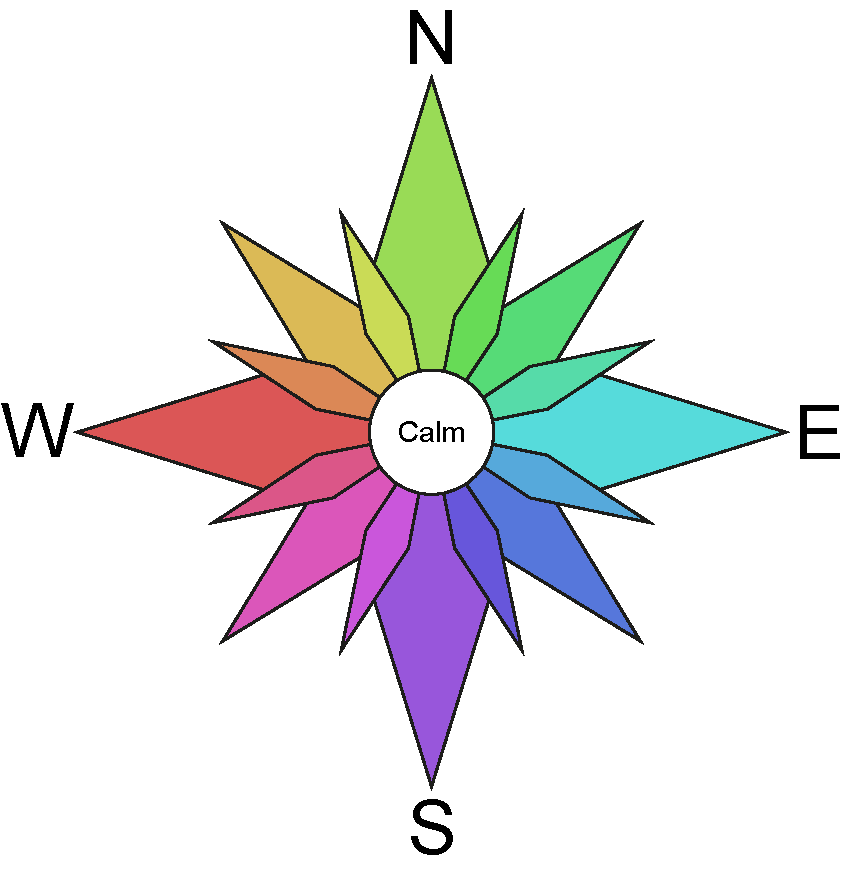
\includegraphics[width=\linewidth]{compass-rose.pdf}
    \caption[Compass Rose mapping colour to wind direction]{
        This compass rose shows the mapping of hue to wind direction used below.
        These colours are equidistant in the HSL colour space, which was rotated
        to avoid a primary red/green contrast in the prevailing monsoon wind.
        }
    \label{fig:compass-rose}
\end{wrapfigure}



Figures \ref{fig:galiwinku-observations} and \ref{fig:milingimbi-observations}
show historical weather observations at Galiwinku and Milingimbi as
sets of heatmaps, where for each variable a grid of year (y) and day-of-year(x)
is shaded according to the observation on that date.
Black cells indicate missing data.
In each figure, the variation in seasonality between years is clearly visible.

Unlike the climographs above, these figures clearly show variation in timing
of seasonal onset between years.  This demonstrates that timeseries data
at daily resolution is required for investigation of Indigenous seasons.


\begin{figure}[p]
    \centering
    \includegraphics[width=\textwidth]{galiwinku/observations.pdf}
    \caption[Historical weather observations at Elcho Island]{
        Historical weather observations at Elcho Island.
        Each panel shows a single variable, with years on the y axis and day-of-year on the x.
        Note that each variable has a different seasonal pattern,
        and that seasonality changes from year to year.}
    \label{fig:galiwinku-observations}
\end{figure}
% Note - if possible, these figures should be on facing pages to allow easy comparison
\begin{figure}[p]
    \centering
    \includegraphics[width=\textwidth]{milingimbi/observations.pdf}
    \caption[Historical weather observations at Milingimbi Airport]{
        Historical weather observations at Milingimbi Airport.
        Each panel shows a single variable, with years on the y axis and day-of-year on the x.
        Note that each variable has a different seasonal pattern,
        and that seasonality changes from year to year.}
    \label{fig:milingimbi-observations}
\end{figure}




\section{Quantifying a Yolngu Calendar}

\subsection{Summary of a Yolngu Calendar}
Following \autoref{ch:seasons}, \autoref{tab:quant-seasons-summary} shows
typical timing and recognition criteria for each season.


\begin{table}[h]
    \centering
    \begin{tabular}{llllll}
        Season          &  Typical Months       &  Criteria to recognise                    \\
        Dhuludur        &  Oct, Nov, Dec        &  Cool at night, mixed wind, first rain    \\
        Barramirri      &  Dec, Jan, Feb        &  NW wind, heavy rain most days            \\
        Mayaltha        &  Feb, Mar             &  NW wind, approx weekly rain              \\
        Midawarr        &  Mar, Apr, May        &  NE to E wind, less rain, last storm      \\
        Dharrathamirri  &  May, Jun, Jul, Aug   &  No rain, consistent ESE-SSE wind         \\
        Rarrandharr     &  Sep, Oct             &  Hot days, low humidity                   
    \end{tabular}
    \caption{A quantifiable summary of the Yolngu seasons case study.}
    \label{tab:quant-seasons-summary}
\end{table}


Additionally, some participants offered tips for recognising seasons,
or information about seasonal patterns.

\begin{itemize}
\item The onset timing of seasons varies between years, with weather conditions. 

\item Seasons can `interrupt' one another, if conditions oscillate appropriately.
        It is however important to avoid premature declarations, so at least two to
        three days of the interrupting season's conditions should be observed.

\item Consequently, seasons may begin and end zero or more times each year -
        and at least once in every annual cycle to date.

\item Seasons are not required to begin in the standard order, though most do.

\item At Galiwinku, and presumably in other coastal locations, the afternoon
        sea breeze obscures the seasonal signal in wind direction.
        9am wind is fine.  3pm is too early.  At various times, 5pm-9pm is best.
        (The analysis below uses 6pm wind for all evening observations.)
\end{itemize}

~\\

TODO - acknowledge importance of these tips and talk about relevance to
detection design.  Will end up in methods.  Most important bit is that
interruption and out-of-order means that forward-filling last known
doesn't work; have to actually check each day.

TODO - with new data, check importance of 3pm/6pm wind, and comment on
whether this makes much difference.




\subsection{Detection of Seasons}
For each season, run detection by the approaches given above.
Present as a multipanel for seach approach, with a panel for each season
and a final full-colour panel for all seasons.  Only provide this for the
Galiwinku data; others can stick to the electronic appendicies.

Discuss briefly which method is considered superior and why; note
that \autoref{ch:analysis} will, to be concise, stick to that one.
The other \emph{may} be used to reproduce results in an appendix.

Close chapter with a table (or similar) presenting seasons, detection
algorithms, and a summary of success rates.  Defer analysis of results
to next chapter.

~\\

There's a lot to do still, but figures \ref{fig:galiwinku-season-counts},
\ref{fig:galiwinku-seasons}, and \ref{fig:milingimbi-seasons}
demonstrate that the concept of the analysis is viable.

\begin{figure}[h]
    \centering
    \includegraphics[width=\textwidth]{galiwinku/season-counts.pdf}
    \caption[Calculated season frequency, Elcho Island]{
        Illustrative count of days for each season, Elcho Island.
        These colours are used for each season in all figures below.
        TODO - make figure smaller
        }
    \label{fig:galiwinku-season-counts}
\end{figure}

\autoref{fig:galiwinku-season-counts} shows the count of days on which
each season was detected.  Like \autoref{fig:compass-rose}, it also
shows the repeated colour scheme.  All other season figures use the
same colour palete, without further labelling.

\autoref{fig:season-index-lines} is very interesting.  TODO EXPLAIN WHY.

\begin{figure}[h]
    \centering
    \includegraphics[width=0.8\textwidth]{galiwinku/seasons-daily-index.pdf}
    \caption[Season index by day-of-year, Elcho Island]{
        Mean normalised (z-score) index for seasons per day-of-year
        at Galiwinku.  Note the clear distinction in the dry season,
        but muddle in the Wet (Dec-Feb).
        This is not indicative of poor detection on a single day,
        but rather that occurence varies more between years.
        }
    \label{fig:season-daily-lines}
\end{figure}


\begin{figure}[h]
    \centering
    \includegraphics[width=0.8\textwidth]{galiwinku/seasons-daily-prob.pdf}
    \caption[Season probability by day-of-year, Elcho Island]{
        Observed probability of each season by day of year.
        }
    \label{fig:season-daily-prob}
\end{figure}




TODO - paragraph referencing and interpreting these figures.

\begin{figure}[p]
    \centering
    \includegraphics[width=\textwidth]{galiwinku/seasons.pdf}
    \caption[Detected seasons for Elcho Island]{
        Detected seasons at Elcho Island, based on hand-crafted threshold conditions.
        DRAFT FIGURE ONLY, will change substantially as method improves.
        }
    \label{fig:galiwinku-seasons}
\end{figure}
% Note - if possible, these figures should be on facing pages to allow easy comparison
\begin{figure}[p]
    \centering
    \includegraphics[width=\textwidth]{milingimbi/seasons.pdf}
    \caption[Detected seasons for Milingimbi Airport]{
        Detected seasons at Milingimbi Airport, based on hand-crafted threshold conditions.
        DRAFT FIGURE ONLY, will change substantially as method improves.
        }
    \label{fig:milingimbi-seasons}
\end{figure}



